\chapter{Järjestelmän tietosisältö}
\section{Käsitekaavio}

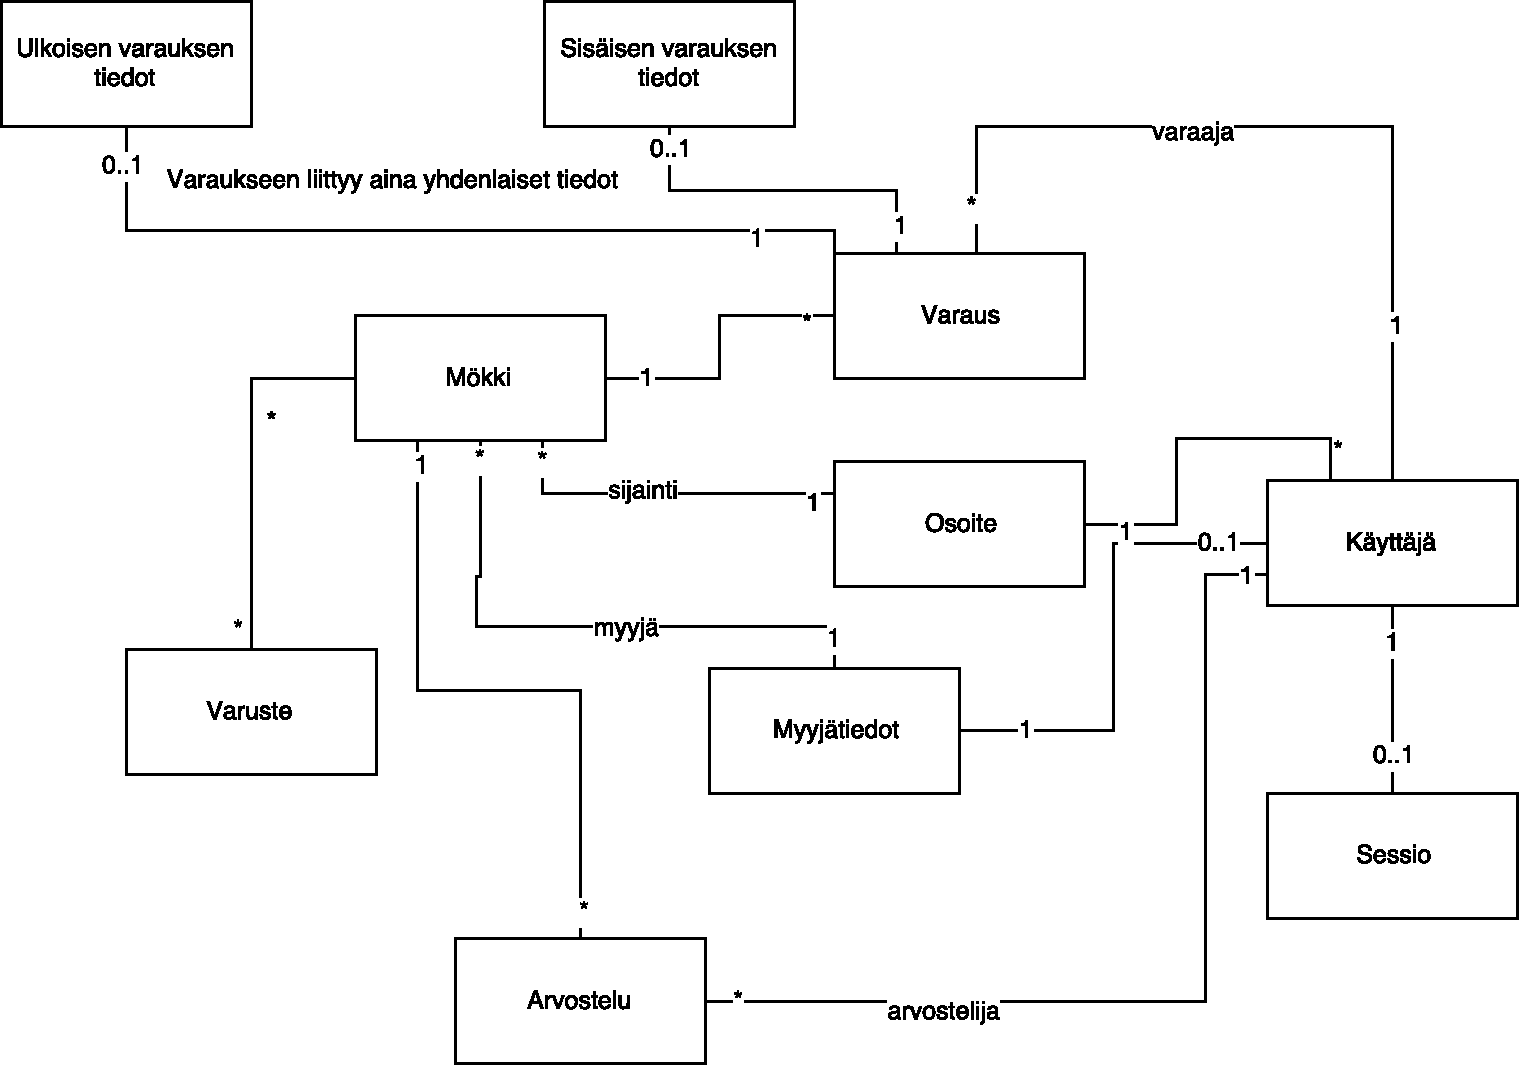
\includegraphics[width = 14cm]{./diagrams/drawio_entities.pdf}
\newpage
\section{Selitteet}
Lähes jokaiseen tietokohteeseen liittyy listattujen ominaisuuksien lisäksi myös uniikki kokonaislukutunniste.

\subsection{Osoite}
Koostuu kahdesta katuosoiterivistä, paikkakunnasta ja postinumerosta. Sisältää myös kaksimerkkisen maakoodin mahdollista laajennusta varten.

\subsection{Käyttäjä}
\begin{tabular}{| l | p{4cm} | p{5cm} |}
	\hline
	Attribuutti & Arvojoukko & Kuvaus \\ \hline
	Rooli & Yksi järjestelmän rooleista & \\ \hline
	Nimi & Rajoittamaton määrä tekstiä & Käyttäjän kutsumanimi. \\ \hline
	Sähköposti & 255 merkkiä tekstiä & \\ \hline
	Salasana & 60 merkkiä tekstiä & BCrypt-salasanatiiviste ja salt. \\ \hline
	Puhelin & Rajoittamaton määrä tekstiä & \\ \hline
	Osoite & Validi viite osoitetauluun & Käyttäjän laskutusosoite. \\ \hline
\end{tabular}

\subsubsection*{Käyttäjäroolit}
\begin{description}
	\item[unverifiedUser] Käyttäjä, jonka sähköpostiosoitetta ei ole vahvistettu.
	\item[user] Tavallinen käyttäjä.
	\item[unapprovedSeller] Vuokranantaja, joka odottaa hyväksyntää.
	\item[seller] Vuokranantaja.
	\item[admin] Järjestelmänvalvoja, joka moderoi sisältöä ja hyväksyy uusia vuokranantajia. 
\end{description}

\subsection{Sessio}
Käyttäjäkohtainen määräaikainen sessio, jota käytetään kirjautumisten tallentamiseen. Sisältää uniikin tunnuksen (32 merkkiä), voimassaoloajan ja käyttäjäviitteen.

\subsection{Myyjätiedot}
Lisätietoa käyttäjään, jos käyttäjä on vahvistettu ja hyväksytty myyjä.

\subsection{Mökki}
\begin{tabular}{| l | p{4cm} | p{5cm} |}
	\hline
	Attribuutti & Arvojoukko & Kuvaus \\ \hline
	Nimi & Rajoittamaton määrä tekstiä & \\ \hline
	Omistaja & Validi viite myyjätietotauluun & \\ \hline
	Osoite & Validi viite osoitetauluun & Mökin sijainti. \\ \hline
	Kuvaus & Rajoittamaton määrä tekstiä & \\ \hline
	Näkyvyys & Tosi tai epätosi & Onko mökki näkyvissä käyttäjille? \\ \hline
	Varauksen alkuaika & Kellonaika & Uusien varausten alkamisaika. \\ \hline
	Varauksen loppumisaika & Kellonaika & Uusien varausten päättymisaika, eli milloin mökki vapautuu. \\ \hline
	Hinta & Kaksidesimaalinen positiivinen luku & Yökohtainen hinta uusille varauksille. \\ \hline
	Pinta-ala & Positiivinen desimaaliluku & Vapaaehtoinen. \\ \hline
	Kerrosten määrä & Positiivinen kokonaisluku & Vapaaehtoinen. \\ \hline
	Rakennusvuosi & Positiivinen kokonaisluku & Vapaaehtoinen. \\ \hline
	Remontointivuosi & Positiivinen kokonaisluku, suurempi tai yhtä suurin kuin rakennusvuosi & Vapaaehtoinen. \\ \hline 
	
\end{tabular}


\subsection{Varuste}
Mökin varuste tai myyntiargumentti \textit{("amenity")}. Kostuu nimestä ja vapaaehtoisesta kuvakkeesta.

\subsection{Varaus}
Varaukseen kuuluu aina tyypistä riippuen joko sisäisen tai ulkoisen varauksen lisätietoja. \\

\begin{tabular}{| l | p{4cm} | p{5cm} |}
	\hline
	Attribuutti & Arvojoukko & Kuvaus \\ \hline
	Mökki & Validi viite mökkitauluun & \\ \hline
	Tyyppi & Varaustyyppi (kts. alla) & \\ \hline
	Varattu aika & Aikaväli, ei saa leikata saman mökin muiden varausten kanssa. & \\ \hline
\end{tabular}

\subsubsection*{Varaustyypit}
\begin{description}
	\item[user] Järjestelmän sisäinen varaus.
	\item[external] Järjestelmän ulkopuolinen varaus.
\end{description}

\subsection{Sisäisen varauksen tiedot}
Lisätietoa varaukseen, jos varaus on tehty järjestelmän sisällä (= sivustolla). Sisältää varaajan käyttäjätunnuksen ja varauksesta maksetun hinnan.

\subsection{Ulkoisen varauksen tiedot}
Lisätietoa varaukseen, jos varaus on tehty järjestelmän ulkopuolella mökin omistajan toimesta (esimerkiksi oman varauksen tai remontin takia). Sisältää selitekentän.

\subsection{Arvostelu}
Arvostelu mökistä. Sisältää arvosanan kokonaislukuna väliltä 1 - 5, mökkitunnuksen, käyttäjätunnuksen ja selitetekstin.